\chapter{Temperatur aus Entropie und Energie}

\lectureoverview{Temperatur tritt zunächst als Umrechnung von Thermometereinheiten des menschlichen Maßstabs in mikroskopische Energieeinheiten auf. Nach der entsprechenden Umrechnung der thermodynamischen Entropie in dimensionslose statistische Entropie beschreiben wir das Gleichgewicht durch eine einparametrige Familie von Wahrscheinlichkeitsverteilungen. Die Ableitung \(dE/dS\) definiert dann die Temperatur, und der erste und der zweite Hauptsatz zeigen, warum eine Temperaturdifferenz die Richtung des Energieflusses bestimmt.}

\section{Umrechnungsfaktoren und menschliche Maßeinheiten}

Viele Konstanten der Physik sind Umrechnungsfaktoren. Die Lichtgeschwindigkeit rechnet eine Länge in eine Zeit um:
\begin{equation}
 t=\frac{x}{c}.
\end{equation}
Misst man Längen und Zeiten in zueinander passenden Einheiten, kann man \(c=1\) setzen. Dadurch verschwindet keine physikalische Wirkung; lediglich beide Messgrößen werden auf dieselbe Skala gebracht.

Die Boltzmann-Konstante hat denselben Charakter. Sie rechnet die auf einem Thermometer im \emph{menschlichen Maßstab} abgelesene Temperatur in eine Energie um. Der Zusatz ist wichtig. Solche Einheiten werden gewählt, weil makroskopische Instrumente sie erzeugen und auflösen können, nicht weil die mikroskopische Dynamik sie auszeichnet.

Das Grad Celsius wurde festgelegt, indem das Intervall zwischen dem Gefrier- und dem Siedepunkt von Wasser bei Normaldruck in hundert Teile geteilt wurde. Die Kelvin-Skala verwendet ein gleich großes Grad, setzt den Nullpunkt aber beim absoluten Nullpunkt an. Die Wahl eines anderen Stoffes, eines anderen Intervalls oder der Fahrenheit-Skala würde die Zahlenwerte, nicht aber die Physik verändern.

\begin{classroomqa}
\audiencequestion{War die Fahrenheit-Skala bereits eine Konstruktion des siebzehnten Jahrhunderts?}
\lecturerresponse{Das genaue Datum ist hier nicht von Bedeutung. Entscheidend ist, dass all diese Skalen für Temperaturen entworfen wurden, die Menschen erzeugen und messen konnten. Die Größe eines Grades ist eine Konvention und keine mikroskopische Vorgabe.
\lecturetimestamp{00:01:34--00:01:50}}
\end{classroomqa}

Als diese Skalen geschaffen wurden, war der molekulare Ursprung der Wärme experimentell noch nicht zugänglich. Eine Änderung um ein Grad ließ sich mit einem makroskopischen Thermometer beobachten, die Energie eines einzelnen Moleküls dagegen nicht messen. Daher lag es nahe, eine Temperatureinheit einzuführen, bevor bekannt war, dass Temperatur im Grunde eine Energieskala ist.

\section{Warum Temperatur die Einheit Energie hat}

Betrachten wir ein verdünntes einatomiges Gas. Verdünnt bedeutet hier, dass die Wechselwirkungsenergien zwischen Molekülen für den vorliegenden Zweck vernachlässigt werden können. Im thermischen Gleichgewicht ordnet das Äquipartitionstheorem jedem quadratischen translatorischen Freiheitsgrad \(T_{\mathrm K}/2\) mal die Boltzmann-Konstante zu. In drei Raumdimensionen gilt
\begin{equation}
 \left\langle E_{\mathrm{kin}}\right\rangle
 =\frac{3}{2}k_{\mathrm B}T_{\mathrm K}.
 \label{eq:sm2-equipartition-kelvin}
\end{equation}
Der Faktor drei zählt die Bewegungen in \(x\)-, \(y\)- und \(z\)-Richtung. Der Faktor ein Halb stammt aus der quadratischen kinetischen Energie.

Diese Beziehung ist nicht auf eine bestimmte Molekülsorte beschränkt. In einem Helium-Sauerstoff-Gemisch hat jedes frei translatorisch bewegliche Teilchen im Gleichgewicht dieselbe mittlere Schwerpunktskinetik, auch wenn sich die schwereren Teilchen langsamer bewegen. Da
\begin{equation}
 E_{\mathrm{kin}}=\frac{1}{2}mv^2,
\end{equation}
folgt aus gleicher charakteristischer Energie \(v\propto m^{-1/2}\).

Dieselbe Idee lässt sich auf ein bewusst extremes Beispiel übertragen. Man hänge eine Bowlingkugel in eine Flüssigkeit und lasse das gesamte System das Gleichgewicht erreichen. Für ihre Brownschen translatorischen Freiheitsgrade gilt dieselbe Energieskala wie für die eines Moleküls. Die Geschwindigkeit der Kugel ist wegen ihrer enorm viel größeren Masse unvorstellbar viel kleiner; die Temperatur vergleicht jedoch Energieskalen, nicht Geschwindigkeiten.

Bei Raumtemperatur beträgt \(T_{\mathrm K}\) etwa \(300\,\mathrm K\), während die Energie eines einzelnen mikroskopischen Freiheitsgrads in Joule winzig ist. Entsprechend klein ist der Umrechnungsfaktor:
\begin{equation}
 k_{\mathrm B}\simeq 1.38\times10^{-23}\,
 \mathrm{J\,K^{-1}}.
 \label{eq:sm2-boltzmann-value}
\end{equation}
Der Zusammenhang zwischen seiner Größenordnung und der Avogadro-Konstante ist kein Zufall:
\begin{equation}
 R=N_{\mathrm A}k_{\mathrm B}.
\end{equation}
Die Gaskonstante \(R\) beschreibt ein Mol, während \(k_{\mathrm B}\) die entsprechende Skala pro mikroskopischem Bestandteil angibt.

In grundlegenden Formeln tritt immer wieder die Kombination \(k_{\mathrm B}T_{\mathrm K}\) auf. Daher ist es übersichtlicher, \begin{equation}
 T\equiv k_{\mathrm B}T_{\mathrm K}.
 \label{eq:sm2-energy-temperature}
\end{equation} zu definieren.
Von nun an hat \(T\) selbst die Einheit einer Energie, und \eqref{eq:sm2-equipartition-kelvin} wird zu
\begin{equation}
 \left\langle E_{\mathrm{kin}}\right\rangle=\frac{3}{2}T.
 \label{eq:sm2-equipartition-natural}
\end{equation}
Misst man Energie in Joule, wird die Temperatur in Joule angegeben. Misst man Energie in Elektronenvolt, wird die Temperatur in Elektronenvolt angegeben. Es gibt keine neue Natureinheit namens Temperatureinheit.

\section{Zwei Konventionen für die Entropie}

Dieselbe Umrechnung tritt auch bei der Entropie auf. Die makroskopische Thermodynamik entwickelte sich aus der Analyse von Wärmekraftmaschinen. Carnot lieferte die entscheidenden Überlegungen zu Wärmekraftmaschinen; Clausius führte später die thermodynamische Entropie und das Symbol \(S\) ein. Bezeichnen wir diese makroskopische Größe in der hier verwendeten Notation mit \(S_{\mathrm C}\). Ihre Einheit ist Energie geteilt durch Thermometertemperatur, beispielsweise Joule pro Kelvin.

Die statistische Entropie ist dimensionslos. Für eine diskrete Verteilung gilt
\begin{equation}
 S=-\sum_i p_i\log p_i.
 \label{eq:sm2-statistical-entropy}
\end{equation}
Bei natürlichen Logarithmen hat eine gleichwahrscheinliche binäre Alternative die Entropie \(\log2\); bei Logarithmen zur Basis zwei wird derselbe Betrag als ein Bit bezeichnet. Die beiden Entropiekonventionen hängen folgendermaßen zusammen:
\begin{equation}
 S=\frac{S_{\mathrm C}}{k_{\mathrm B}},
 \qquad
 S_{\mathrm C}=k_{\mathrm B}S.
 \label{eq:sm2-entropy-conversion}
\end{equation}
Ein makroskopischer Wert, der in \(\mathrm{J\,K^{-1}}\) bescheiden erscheint, entspricht einer enormen dimensionslosen Entropie, denn diese zählt die Information, die auf eine enorme Zahl mikroskopischer Bestandteile verteilt ist.

Die Gleichungen \eqref{eq:sm2-energy-temperature} und \eqref{eq:sm2-entropy-conversion} legen die durchgehend verwendete Konvention fest:
\[
 [T]=[\text{energy}],
 \qquad
 [S]=1.
\]
Die Boltzmann-Konstante kann nun aus den Arbeitsformeln verschwinden. Sie lässt sich jederzeit wieder einsetzen, indem man \(T\) durch \(k_{\mathrm B}T_{\mathrm K}\) und \(S\) durch \(S_{\mathrm C}/k_{\mathrm B}\) ersetzt.

\begin{classroomqa}
\audiencequestion{Ist die neue Temperatur abgesehen vom Faktor \(3/2\) einfach eine in Joule gemessene Energie?}
\lecturerresponse{Ja, sofern Joule als Energieeinheit gewählt wird. Ein Joule ist die MKS-Einheit \(\mathrm{kg\,m^2\,s^{-2}}\). Man könnte stattdessen Elektronenvolt oder eine andere Energieeinheit verwenden; dann muss die Temperatur in derselben Einheit angegeben werden. Der Faktor \(3/2\) gehört zum Beispiel des idealen Gases, nicht zur Definition der Temperatur.
\lecturetimestamp{00:15:49--00:16:45}}
\end{classroomqa}

\begin{classroomqa}
\audiencequestion{Wenn die Tafel Kelvin vorgibt, ist \(k_{\mathrm B}\) dann nicht eine festgelegte Konstante?}
\lecturerresponse{Sie ist festgelegt, sobald sowohl die Temperatur- als auch die Energieeinheit angegeben sind. Wechselt man von Kelvin zu Fahrenheitgraden oder von Joule zu Elektronenvolt, ändert sich ihr Zahlenwert. Genau so muss sich ein Umrechnungsfaktor mit der Einheit ändern.
\lecturetimestamp{00:16:46--00:18:33}}
\end{classroomqa}

\begin{classroomqa}
\audiencequestion{Wird der Zahlenwert der Boltzmann-Konstante experimentell bestimmt?}
\lecturerresponse{Ja. Historisch erforderte ihre Bestimmung mikroskopische Informationen über Atome und deren Teilchendichte. Boltzmann verstand den Zusammenhang zwischen Molekülenergie und Temperatur, bevor diese Größen genau bekannt waren – ähnlich wie Newton die Rolle der Gravitationskonstante kannte, bevor sie präzise gemessen worden war.
\lecturetimestamp{00:18:46--00:20:00}}
\end{classroomqa}

\section{Gleichgewicht ist ein statistischer Zustand}

Die Einheitenumrechnung hat die Temperatur noch immer nicht definiert. Etwas Heißes zu berühren vermittelt eine nützliche biologische Intuition, doch Temperatur ist eine abgeleitete physikalische Größe, die aus Energie und Entropie gebildet wird.

Man stelle sich ein System vor, das mit einer großen Umgebung in Kontakt steht, deren makroskopische Bedingungen festgehalten werden. Energie kann zwischen beiden ausgetauscht werden. Hat das System anfangs zu viel Energie, gibt es im Mittel Energie ab; hat es zu wenig, nimmt es im Mittel Energie auf. Im thermischen Gleichgewicht finden weiterhin mikroskopische Austauschvorgänge statt, doch im Mittel gibt es keinen Nettofluss in eine der beiden Richtungen.

Bezeichne \(i\) einen exakten mikroskopischen Zustand des Systems und \(E_i\) dessen Energie. Gleichgewicht bedeutet nicht, dass das System in einem Zustand erstarrt. Seine Wechselwirkung mit der Umgebung verändert den Mikrozustand fortwährend, daher ordnen wir jeder Möglichkeit eine Wahrscheinlichkeit \(P_i\) zu. Die grundlegenden Beziehungen lauten
\begin{align}
 \sum_i P_i &=1,
 \label{eq:sm2-normalization}\\
 \sum_i P_iE_i &=\overline E,
 \label{eq:sm2-mean-energy}\\
 S&=-\sum_iP_i\log P_i.
 \label{eq:sm2-equilibrium-entropy}
\end{align}
Der Balken über \(\overline E\) hebt hervor, dass die Energie des Teilsystems schwankt. Eine Messung kann einen Wert ergeben, die nächste einen anderen; bei wiederholten Messungen ergibt sich die Verteilung, deren Mittelwert \eqref{eq:sm2-mean-energy} ist.

\begin{figure}[t]
\centering
\includegraphics[width=0.82\textwidth]{lecture_02_figure_02.png}
\caption{Normierung und mittlere Energie an der Tafel: \(\sum_iP(i)=1\) und \(\sum_iP(i)E(i)=\langle E\rangle\).}
\lectureframe{00:24:10}
\end{figure}

\section{Eine durch die mittlere Energie parametrisierte Familie}

Die Gleichgewichtsverteilung hängt stark von der mittleren Energie ab. Stellt man einen Topf Wasser auf den Herd, steigt \(\overline E\); stellt man ihn in den Schnee, sinkt \(\overline E\). Die Wahrscheinlichkeiten ändern sich entsprechend. Gleichgewicht sollte daher nicht als eine einzelne Verteilung, sondern als einparametrige Familie betrachtet werden:
\begin{equation}
 P_i(\overline E).
 \label{eq:sm2-family}
\end{equation}
Jedes Familienmitglied erfüllt
\begin{align}
 \sum_iP_i(\overline E)&=1,
 \label{eq:sm2-family-normalization}\\
 \sum_iP_i(\overline E)E_i&=\overline E.
 \label{eq:sm2-family-mean}
\end{align}

\begin{figure}[t]
\centering
\includegraphics[width=0.88\textwidth]{lecture_02_figure_03.png}
\caption{Der Übergang zu \(P(i,\overline E)\). Die vorherigen Gleichungen für Normierung, mittlere Energie und Entropie bleiben sichtbar, während die Verteilungsfamilie eingeführt wird.}
\lectureframe{00:26:29}
\end{figure}

Für eine schematische Darstellung ordnen wir die Zustände nach aufsteigendem \(E_i\). Die horizontale Achse kann dann entweder als Index \(i\) oder als zugehörige Energie gelesen werden. Bei größerer mittlerer Energie verschiebt sich das Wahrscheinlichkeitsgewicht zu weiter rechts liegenden Zuständen. Die Gesamtfläche unter jeder Kurve muss weiterhin eins betragen.

\begin{figure}[t]
\centering
\includegraphics[width=0.88\textwidth]{lecture_02_figure_04.png}
\caption{Mehrere schematische Verteilungen \(P(i,\overline E)\). Kurven, deren Gewicht weiter rechts liegt, haben eine größere mittlere Energie; jede bleibt normiert.}
\lectureframe{00:28:40}
\end{figure}

\begin{figure}[t]
\centering
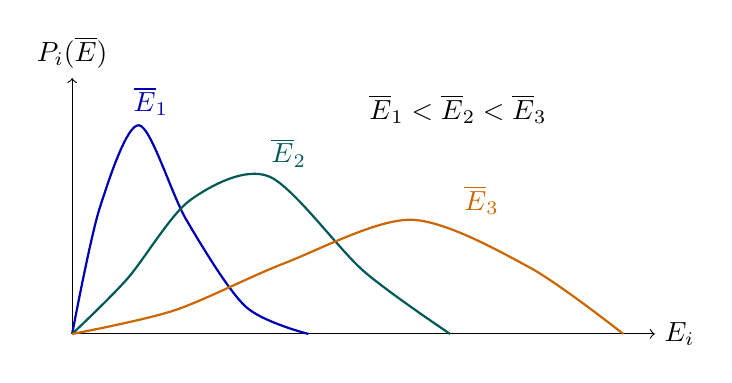
\begin{tikzpicture}[x=1cm,y=1cm]
\draw[->] (0,0) -- (7.4,0) node[right] {$E_i$};
\draw[->] (0,0) -- (0,3.25) node[above] {$P_i(\overline E)$};
\draw[thick,blue!70!black]
  plot[smooth] coordinates {(0,0) (0.35,1.6) (0.85,2.65) (1.45,1.45)
  (2.2,0.35) (3.0,0)};
\draw[thick,teal!70!black]
  plot[smooth] coordinates {(0,0) (0.7,0.7) (1.5,1.7) (2.5,2.0)
  (3.7,0.8) (4.8,0)};
\draw[thick,orange!80!black]
  plot[smooth] coordinates {(0,0) (1.3,0.3) (2.7,0.9) (4.3,1.45)
  (5.8,0.85) (7.0,0)};
\node[blue!70!black] at (1.0,2.95) {\(\overline E_1\)};
\node[teal!70!black] at (2.75,2.3) {\(\overline E_2\)};
\node[orange!80!black] at (5.2,1.7) {\(\overline E_3\)};
\node at (4.9,2.85) {\(\overline E_1<\overline E_2<\overline E_3\)};
\end{tikzpicture}
\caption{Eine bereinigte Fassung der Skizze an der Tafel. Die Kurven müssen nicht genau diese Formen haben; berücksichtigt werden lediglich die Normierung und die aufsteigend geordneten mittleren Energien.}
\end{figure}

\begin{classroomqa}
\audiencequestion{Ist die Notation zirkulär? Die mittlere Energie wird aus der Verteilung berechnet, während die Verteilung durch die mittlere Energie parametrisiert wird.}
\lecturerresponse{Man beginne mit einer empirisch ausgewählten einparametrigen Familie von Gleichgewichtsverteilungen. Jedes Familienmitglied hat eine mittlere Energie. Haben verschiedene Mitglieder verschiedene Mittelwerte, kann dieser Mittelwert als Parameter dienen, der die Familie bezeichnet. Die Notation leitet die Familie noch nicht her; diese Herleitung wird später durch die Boltzmann-Verteilung geliefert.
\lecturetimestamp{00:28:35--00:29:44}}
\end{classroomqa}

\begin{classroomqa}
\audiencequestion{Warum spricht man von mittlerer Energie statt von Gesamtenergie?}
\lecturerresponse{Das Teilsystem tauscht Energie mit einem Wärmebad aus, etwa mit der Atmosphäre, die einen Gasbehälter mit thermisch durchlässigen Wänden umgibt. Seine momentane Energie schwankt. Viele Messungen ergeben eine Verteilung, und \(\overline E\) ist der Mittelwert dieser Messwerte. Die Energie des größeren abgeschlossenen Systems aus Teilsystem und Wärmebad kann dennoch konstant sein.
\lecturetimestamp{00:29:46--00:30:56}}
\end{classroomqa}

\begin{classroomqa}
\audiencequestion{Können verschiedene mikroskopische Zustände dieselbe Energie und verschiedene Verteilungen dieselbe mittlere Energie haben?}
\lecturerresponse{Beides ist möglich. Die Nebenbedingung an die mittlere Energie allein lässt viele Verteilungen zu; die besondere einparametrige Gleichgewichtsfamilie erfordert daher ein zusätzliches physikalisches Argument. Ihr Ursprung und ihre Boltzmann-Form werden später hergeleitet. Gleiche Energien verschiedener Mikrozustände sind die davon getrennte Frage der Entartung.
\lecturetimestamp{00:30:58--00:32:22}}
\end{classroomqa}

\subsection{Zustandsbezeichnungen, Entartung und Korrelation}

Mehrere leicht zu vermischende Unterscheidungen müssen auseinandergehalten werden.

Erstens können viele Wahrscheinlichkeitsverteilungen dieselbe mittlere Energie haben. Die einparametrige Gleichgewichtsfamilie folgt nicht allein aus der Nebenbedingung an die mittlere Energie. Es handelt sich um die spezielle Familie, die durch die Einstellung des Gleichgewichts ausgewählt wird; ihre Form wird später als Boltzmann-Verteilung identifiziert.

Zweitens können mehrere verschiedene Mikrozustände dieselbe Energie haben. Das nennt man Entartung. In der Diskussion an der Tafel werden exakte Entartungen vorübergehend ignoriert, damit sich die Zustände eindeutig nach Energie ordnen lassen. Entartung kommt bei Systemen mit Symmetrien tatsächlich häufig vor, bereitet aber begrifflich kein Problem: Man behält die Zustandsbezeichnung \(i\) bei, lässt wiederholte Werte von \(E_i\) zu und summiert über alle Zustände.

Drittens ist Korrelation kein anderes Wort für Entartung. Korrelation betrifft eine gemeinsame Verteilung zweier Zufallsgrößen und fragt, ob die Kenntnis der einen die Wahrscheinlichkeiten für die andere verändert. Die sich gegenseitig ausschließenden Bezeichnungen \(i\) und \(j\) in einer Liste von Mikrozuständen sind für sich genommen keine zwei Zufallsvariablen, deren Korrelation berechnet wird.

\begin{classroomqa}
\audiencequestion{Setzt die Konstruktion voraus, dass verschiedene \(i\)-Zustände unabhängig sind, und was ist, wenn zwei davon korreliert sind?}
\lecturerresponse{Eine Zustandsbezeichnung ist ein möglicher Wert ein und derselben mikroskopischen Zufallsvariablen. Unabhängigkeit und Korrelation erfordern zwei gemeinsam verteilte Variablen; diese Begriffe lassen sich daher nicht unmittelbar auf zwei alternative Bezeichnungen in dieser Liste anwenden. Gleiche Energien verschiedener Zustände betreffen stattdessen die Entartung.
\lecturetimestamp{00:32:23--00:33:22}}
\end{classroomqa}

\begin{classroomqa}
\audiencequestion{Was ist, wenn zwei verschiedene Zustände genau dieselbe Energie haben?}
\lecturerresponse{Das ist Entartung. Für die unmittelbare grafische Darstellung treffen wir die vereinfachende Annahme, dass keine zwei Energien übereinstimmen, und ordnen die Zustände nach aufsteigender Energie. Die späteren Wahrscheinlichkeitsformeln erfordern diese Annahme nicht; entartete Zustände werden einfach einzeln gezählt.
\lecturetimestamp{00:33:23--00:34:04}}
\end{classroomqa}

\begin{classroomqa}
\audiencequestion{Ist die Bedeutung des Index \(i\) beliebig?}
\lecturerresponse{Die mikroskopischen Zustände selbst sind nicht beliebig: Jeder legt alle Positionen, Impulse oder sonstigen Daten fest, die für eine exakte Beschreibung nötig sind. Beliebig sind ihre Namen. Für die Abbildung wählen wir daher Bezeichnungen, die nach Energie aufsteigend geordnet sind.
\lecturetimestamp{00:34:06--00:35:15}}
\end{classroomqa}

\section{Entropie wird zu einer Funktion der Energie}

Jedes Mitglied der Gleichgewichtsfamilie hat eine Entropie. Setzt man \eqref{eq:sm2-family} in \eqref{eq:sm2-equilibrium-entropy} ein, erhält man
\begin{equation}
 S(\overline E)
 =-\sum_iP_i(\overline E)\log P_i(\overline E).
 \label{eq:sm2-entropy-energy}
\end{equation}
Dies ist keine universelle Funktion, die für alle physikalischen Systeme gilt. Sie hängt vom Spektrum des Systems und seiner Gleichgewichtsfamilie ab. Ist diese Familie jedoch festgelegt, sind Energie und Entropie miteinander verknüpft: Bewegt man sich innerhalb der Familie, ändern sich beide.

In gewöhnlichen Systemen verteilt sich die Wahrscheinlichkeit typischerweise mit steigender mittlerer Energie auf mehr Zustände, sodass \(S\) gewöhnlich mit \(\overline E\) zunimmt. Vorläufig nehmen wir an, dass dieser Zusammenhang glatt und lokal umkehrbar ist. Die Ausnahmen sind wichtig, doch der einfache Fall macht die benötigte Definition sichtbar.

\section{Die Ableitung, die Temperatur definiert}

Stellen wir eine konkrete Frage: Um wie viel muss sich die mittlere Energie ändern, damit die Entropie um eine binäre Alternative zunimmt? In Einheiten des natürlichen Logarithmus beträgt dieser Entropiezuwachs \(\log2\).

Für benachbarte Mitglieder einer glatten Familie gilt
\begin{equation}
 dE=\frac{dE}{dS}\,dS.
 \label{eq:sm2-differential-identity}
\end{equation}
An dieser Stelle ist die Gleichung lediglich die Kettenregel. Ihr Koeffizient hat jedoch genau die Dimensionen und die physikalische Rolle, die für eine Temperatur erforderlich sind.

\begin{definition}
Die Temperatur in Energieeinheiten ist
\begin{equation}
 T\equiv\frac{dE}{dS}.
 \label{eq:sm2-temperature-definition}
\end{equation}
Äquivalent dazu gilt
\begin{equation}
 dE=T\,dS,
 \qquad
 dS=\frac{1}{T}\,dE.
 \label{eq:sm2-fundamental-differentials}
\end{equation}
\end{definition}

Für eine hinreichend kleine Änderung um ein Bit gilt
\begin{equation}
 \Delta E\simeq T\log2.
 \label{eq:sm2-one-bit-energy}
\end{equation}
Die Beschränkung auf ein Bit dient nur dazu, die Ableitung anschaulich zu machen. Für jede kleine Entropieänderung gilt dieselbe lokale Beziehung.

\begin{classroomqa}
\audiencequestion{Da die Entropie als \(S(E)\) geschrieben wurde, wäre dann \(dS/dE\) nicht die natürlichere Ableitung?}
\lecturerresponse{Bei lokal umkehrbarem Zusammenhang enthalten beide Ableitungen dieselbe Information:
\[
 \frac{dE}{dS}=\left(\frac{dS}{dE}\right)^{-1}.
\]
Als Temperatur bezeichnet man konventionell \(dE/dS\), während die inverse Temperatur \(dS/dE=1/T\) ist.
\lecturetimestamp{00:40:24--00:40:54}}
\end{classroomqa}

Hier ändert sich nur eine thermodynamische Variable, daher genügen gewöhnliche Ableitungen. Können sich Volumen, Teilchenzahl, Magnetisierung oder andere Variablen ändern, muss man partielle Ableitungen verwenden und angeben, welche Größen konstant gehalten werden. Die vorliegende Definition ist der eindimensionale Schnitt durch diese allgemeinere thermodynamische Geometrie.

\subsection{Warum sich die Boltzmann-Konstante herauskürzt}

Kehren wir kurz zu den Thermometereinheiten zurück. Mit
\[
 T=k_{\mathrm B}T_{\mathrm K},
 \qquad
 S=\frac{S_{\mathrm C}}{k_{\mathrm B}},
\]
lautet die grundlegende Beziehung
\begin{align}
 dE
 &=\bigl(k_{\mathrm B}T_{\mathrm K}\bigr)
   d\left(\frac{S_{\mathrm C}}{k_{\mathrm B}}\right)\\
 &=T_{\mathrm K}\,dS_{\mathrm C}.
 \label{eq:sm2-carnot-form}
\end{align}
Ein Faktor \(k_{\mathrm B}\) tritt über die Temperatur ein, der Kehrwert desselben Faktors über die Entropie. Beide kürzen sich heraus. Deshalb kann ein Lehrbuch der konventionellen Thermodynamik \eqref{eq:sm2-carnot-form} schreiben, ohne die Boltzmann-Konstante anzugeben.

\begin{classroomqa}
\audiencequestion{Muss \(S(E)\) umkehrbar sein?}
\lecturerresponse{Nicht immer. Bei gewöhnlichen Systemen im hier betrachteten Bereich verbreitert sich die Gleichgewichtsverteilung mit zunehmender Energie im Allgemeinen, und die Entropie nimmt zu. Daher ist \(S(E)\) monoton und \(T>0\). Systeme mit beschränkten Spektren können Gegenbeispiele liefern, darunter Bereiche, in denen die Entropie mit der Energie abnimmt und die statistische Temperatur negativ ist. Diese Fälle lassen wir vorerst beiseite.
\lecturetimestamp{00:44:30--00:45:57}}
\end{classroomqa}

\section{Von der abstrakten Ableitung zu heiß und kalt}

Die Ableitungsdefinition ist universell, aber noch abstrakt. Wir möchten die vertraute Aussage herleiten, dass Energie von einem wärmeren Körper zu einem kälteren fließt. Der Schmerz beim Berühren einer heißen Oberfläche ist biologischer Natur; Farbe und ausgesandte Strahlung hängen von den Eigenschaften des Lichts ab. Eine statistische Definition sollte auch für ein idealisiertes Gas sinnvoll sein, wenn Strahlung außer Acht gelassen wird.

\begin{classroomqa}
\audiencequestion{Könnte die von einem heißen Gegenstand ausgesandte Strahlung als grundlegende Definition der Temperatur dienen?}
\lecturerresponse{Strahlung ist ein nützliches Thermometer, bringt aber die Physik des Lichts ins Spiel. Die statistische Mechanik muss Temperatur für Systeme wie einen Gaskasten definieren können, ohne sich auf optische Eigenschaften zu stützen. Die Richtung des Energieaustauschs ist das allgemeinere Kriterium.
\lecturetimestamp{00:46:42--00:47:20}}
\end{classroomqa}

Man bereite zwei Systeme \(A\) und \(B\) vor, die sich zunächst jeweils in ihrem eigenen Gleichgewicht befinden und die Temperaturen \(T_A\) und \(T_B\) haben. Anfangs sind sie voneinander isoliert. Dann verbinde man sie durch einen schwachen thermischen Kontakt: Das \emph{dünne Rohr} lässt kleine Energiemengen hin und her fließen, ohne die Identität der beiden Teilsysteme aufzuheben.

\begin{figure}[t]
\centering
\includegraphics[width=0.88\textwidth]{lecture_02_figure_05.png}
\caption{Die getrennt vorbereiteten Systeme \(A\) und \(B\) mit den Temperaturen \(T_A\) und \(T_B\), bevor der schwache thermische Kontakt betrachtet wird.}
\lectureframe{00:48:55}
\end{figure}

\begin{figure}[t]
\centering
\begin{tikzpicture}[>=Stealth]
\draw[rounded corners,thick,fill=blue!6] (0,0) rectangle (2.6,2.4);
\draw[rounded corners,thick,fill=orange!8] (5.4,0) rectangle (8,2.4);
\draw[thick] (2.6,1.35) -- (5.4,1.35);
\draw[thick] (2.6,1.05) -- (5.4,1.05);
\draw[<->,very thick] (3.15,1.2) -- (4.85,1.2)
  node[midway,above] {\(\delta E\)};
\node at (1.3,1.45) {\Large \(A\)};
\node at (6.7,1.45) {\Large \(B\)};
\node at (1.3,0.65) {\(T_A,S_A,E_A\)};
\node at (6.7,0.65) {\(T_B,S_B,E_B\)};
\node at (4,0.35) {\small weak thermal contact};
\end{tikzpicture}
\caption{Energie fluktuiert durch den schwachen Kontakt, während das Gesamtsystem isoliert bleibt.}
\end{figure}

Nehmen wir ohne Beschränkung der Allgemeinheit an,
\begin{equation}
 T_B>T_A.
 \label{eq:sm2-temperature-order}
\end{equation}
Erfahrungsgemäß sollte \(B\) Energie abgeben und \(A\) Energie aufnehmen. Drei Tatsachen führen diese Erwartung auf eine Rechnung zurück.

\subsection{Additivität der Entropie}

Bei zwei schwach gekoppelten Teilsystemen, deren mikroskopische Alternativen sich unabhängig kombinieren, multipliziert sich die Zahl der gemeinsamen Möglichkeiten:
\[
 W_{AB}=W_AW_B.
\]
Die Entropie ist logarithmisch, also gilt
\begin{equation}
 S_{\mathrm{tot}}=S_A+S_B.
 \label{eq:sm2-entropy-additivity}
\end{equation}
Dasselbe Ergebnis folgt unmittelbar aus der Shannon-Entropie einer Produktverteilung.

\begin{classroomqa}
\classquestion{Warum addieren sich die Entropien der Gesamtsysteme?}
\lecturerresponse{Weil sich die zugrunde liegenden Anzahlen der Alternativen multiplizieren, während die Entropie den Logarithmus bildet:
\(\log(W_AW_B)=\log W_A+\log W_B\). Die schwache Wechselwirkung ermöglicht die Beschreibung durch Teilsysteme und diese additive Näherung erster Ordnung.
\lecturetimestamp{00:51:06--00:52:03}}
\end{classroomqa}

\subsection{Der erste und der zweite Hauptsatz}

Das Gesamtsystem ist isoliert; daher bleibt die intern ausgetauschte Energie erhalten:
\begin{equation}
 dE_A+dE_B=0,
 \qquad
 dE_B=-dE_A.
 \label{eq:sm2-first-law}
\end{equation}
Dies ist der erste Hauptsatz für das vorliegende Experiment.

Den zweiten Hauptsatz setzen wir hier als Postulat voraus; seine tiefere Begründung folgt später. Während sich die verbundenen Systeme auf ihr neues Gleichgewicht einstellen,
\begin{equation}
 dS_{\mathrm{tot}}=dS_A+dS_B\geq0.
 \label{eq:sm2-second-law}
\end{equation}
Die strikte Ungleichung beschreibt die spontane Relaxation aus dem Gleichgewicht heraus; im Gleichgewicht gilt bei einer reversiblen Variation erster Ordnung Gleichheit.

Schließlich gilt die Temperaturdefinition für jedes Teilsystem:
\begin{equation}
 dE_A=T_A\,dS_A,
 \qquad
 dE_B=T_B\,dS_B.
 \label{eq:sm2-two-temperatures}
\end{equation}

\begin{figure}[H]
\centering
\includegraphics[width=0.88\textwidth]{lecture_02_figure_06.png}
\caption{Die Beziehungen für die beiden Teilsysteme
\(dE_A=T_A\,dS_A\) und \(dE_B=T_B\,dS_B\) am Ende der Argumentation an der Tafel.}
\lectureframe{00:54:00}
\end{figure}

\subsection{Das Vorzeichen des Energieflusses}

Diese Gleichungen legen die Richtung des Nettoenergietransfers bereits fest. Setzen wir \(dS_A=dE_A/T_A\), \(dS_B=dE_B/T_B\) und \eqref{eq:sm2-first-law} in \eqref{eq:sm2-second-law} ein:
\begin{align}
 dS_{\mathrm{tot}}
 &=\frac{dE_A}{T_A}+\frac{dE_B}{T_B}\\
 &=dE_A\left(\frac{1}{T_A}-\frac{1}{T_B}\right)\geq0.
 \label{eq:sm2-flow-sign}
\end{align}
Wenn \(T_B>T_A>0\) gilt, dann
\[
 \frac{1}{T_A}-\frac{1}{T_B}>0.
\]
Daher erfordert Gleichung \eqref{eq:sm2-flow-sign}
\[
 dE_A>0,
 \qquad
 dE_B<0.
\]
Das kältere System \(A\) nimmt Energie auf, und das wärmere System \(B\) gibt Energie ab. Wenn \(T_A=T_B\) gilt, gibt es für die Entropieänderung erster Ordnung keine bevorzugte Richtung, und die mikroskopischen Austauschvorgänge gleichen sich zu einem Nettofluss von null aus. Somit bildet die abstrakte Ableitung \(T=dE/dS\) den operationellen Unterschied zwischen warm und kalt ab.